% IFAS: Intelligent Footfall Analysis System for Retail Environments
%
% Build:   tectonic ifas.tex        (or upload this folder to Overleaf)
% Figures: python figures/make_figures.py   regenerates every plot
\documentclass[conference]{IEEEtran}

\usepackage[T1]{fontenc}
\usepackage[utf8]{inputenc}
\usepackage{microtype}
\usepackage{cite}
\usepackage{amsmath,amssymb}
\usepackage{graphicx}
\usepackage{booktabs}
\usepackage{array}
\usepackage{xcolor}
\usepackage{algorithm}
\usepackage{algpseudocode}
\usepackage{tikz}
\usetikzlibrary{arrows.meta,chains,positioning,decorations.pathreplacing,calc}
\usepackage[hidelinks]{hyperref}

\graphicspath{{figures/}}

% Diagram colours match the plots: blue for the learned network, orange for
% the classical model, ink for everything else.
\definecolor{ink}{HTML}{1B1F3B}
\definecolor{cool}{HTML}{2A6FDC}
\definecolor{warm}{HTML}{E0602A}

\tikzset{
  >=Stealth,
  box/.style={draw=ink!65, line width=0.5pt, rounded corners=2.5pt, fill=white,
    align=center, inner xsep=4.5pt, inner ysep=4pt, minimum height=10mm,
    font=\footnotesize, text=ink},
  deep/.style={box, draw=cool!85, fill=cool!9},
  classic/.style={box, draw=warm!90, fill=warm!11},
  flow/.style={->, line width=0.55pt, draw=ink!75},
  note/.style={font=\scriptsize, text=ink!80},
  span/.style={decorate, decoration={brace, mirror, amplitude=4pt}, line width=0.45pt, draw=ink!60},
}

\newcommand{\mA}{\mathrm{mA}}
\newcommand{\sci}[1]{$10^{#1}$}
\renewcommand{\algorithmicrequire}{\textbf{Input:}}
\renewcommand{\algorithmicensure}{\textbf{Output:}}

% Stage timings, copied from figures/runtime.json (scripts/benchmark_stages.py).
\newcommand{\tDetect}{157}       % ms per frame
\newcommand{\tGender}{794}       % ms per crop, batch of 16
\newcommand{\tGenderOne}{900} % ms per crop, batch of 1
\newcommand{\tAge}{55}             % ms per crop
\newcommand{\tAgeFeat}{43}     % ms per crop, histograms only
\newcommand{\tPerson}{12}       % upper bound in seconds: 12 votes x (900 + 55) ms

\begin{document}

\title{IFAS: Intelligent Footfall Analysis System\\for Retail Environments}

\author{\IEEEauthorblockN{Abhishek Pandey, Devendra Mote, Rishi Popawala and Yash Dave}
\IEEEauthorblockA{Department of Information Technology\\
Dwarkadas J. Sanghvi College of Engineering, Mumbai, Maharashtra, India\\
Project guide: Prof. Neha Katre}
\thanks{All authors contributed equally to this work.}}

\maketitle

\begin{abstract}
Retail stores record hours of camera footage every day and use almost none of it.
This paper presents IFAS, a system that turns that footage into a count of visitors
with their gender, their age group, the time they stay and the places they stand.
IFAS gives each task the simplest model that does it well. A YOLOv8 detector finds
people and an IoU tracker follows them across frames. A ViT-B/16 network classifies
gender after transfer learning on the PETA dataset. Four support vector machines
classify age from colour and texture histograms, following the original PETA
benchmark. Each person is classified on several frames and the results are pooled
into one label. In our study the gender model reaches 97.8\% validation accuracy on
PETA. On the PETA test split the age model reaches a mean accuracy of 0.835 over
four age groups and a four-way accuracy of 76.7\%. Four out of five of its errors
land in a neighbouring age group. We report how sensitive both models are to their
main settings and how long each stage takes on a laptop processor. A check on
shop footage shows where detection and tracking fail and how far two additions,
rejoining lost tracks and a second detector for weak detections, repair it.
\end{abstract}

\begin{IEEEkeywords}
footfall analysis, pedestrian attribute recognition, vision transformer, transfer
learning, support vector machine, local binary patterns, retail analytics
\end{IEEEkeywords}

% ---------------------------------------------------------------------------
\section{Introduction}

A store that wants to know how many people came in today has two options. It can
post someone at the door with a clicker or it can read the number off a sensor
above the entrance. Neither says who came in, how long they stayed or where they
stood. The cameras that already watch the shop floor record all of that, and
almost none of it is used.

Reading the footage by hand does not scale. One person can watch one screen, and
a manual count drifts after a few minutes. A store with eight cameras and a
twelve hour day produces close to a hundred hours of video a day. The work has to
be automated before the footage is worth keeping.

This paper describes IFAS, the Intelligent Footfall Analysis System. IFAS takes a
recorded video and returns a record of every person who appears in it. The record
holds the person's gender and age group, the time they entered and left the frame
and the path they took. A dashboard reads these records and shows them as counts,
charts and a short written summary.

The design follows one rule: each task gets the simplest model that does it well.
Gender is a binary label with plenty of training data, so a pretrained vision
transformer~\cite{dosovitskiy2021vit} is a good fit. We fine-tune ViT-B/16 in two
stages. The first uses the public PETA dataset~\cite{deng2014peta} and the second
adapts the model to footage from the target store. Age is harder to read from a
pedestrian crop, and PETA has few examples in some age groups. For age we follow
the original PETA benchmark~\cite{deng2014peta} and train one support vector
machine per age group on colour and texture histograms. This keeps the age results
comparable with the published baseline. Detection needs speed more than depth, so
a small YOLOv8 model~\cite{jocher2023yolov8} does that job.

The contributions of this work are as follows.
\begin{itemize}
  \item A pipeline that joins detection, tracking and two attribute classifiers
        and pools several predictions per person into one label.
  \item A sensitivity study of four training settings for the gender model and
        five feature settings for the age model.
  \item A full evaluation of the age model on the PETA test split, with an
        analysis of where its errors fall.
  \item Timings of every stage on a laptop processor, and the per-person cost
        bound that follows from them.
  \item A tracker that rejoins people the detector loses, and a second detector
        that is consulted only about weak detections, with a field check that
        shows what each one fixes.
\end{itemize}

Section~\ref{sec:related} reviews related work. Section~\ref{sec:system}
describes the system. Section~\ref{sec:experiments} reports the experiments.
Section~\ref{sec:discussion} discusses the results and their limits, and
Section~\ref{sec:conclusion} concludes.

% ---------------------------------------------------------------------------
\section{Related Work}
\label{sec:related}

\subsection{Pedestrian Attribute Recognition}
Deng et al.~\cite{deng2014peta} introduced the PEdesTrian Attribute (PETA)
dataset. It joins ten smaller surveillance datasets into 19,000 images labelled
with 61 binary attributes and four multi-class attributes. Gender and age group
are among them. Their baseline describes each image with colour and texture
features and trains one SVM per attribute. Each attribute is scored by mean
accuracy, the average of the accuracy on positive examples and the accuracy on
negative examples. A classifier that always predicts the majority class gains
nothing under this measure. Later work on pedestrian attributes reports the same
measure, and so do we.

\subsection{Vision Transformers}
The transformer~\cite{vaswani2017attention} was designed for text. Dosovitskiy et
al.~\cite{dosovitskiy2021vit} applied it to images by cutting each image into
patches of $16\times16$ pixels and treating the patches as a sequence. Their
Vision Transformer (ViT) matches or beats convolutional networks when it is
pretrained on a large dataset such as ImageNet-21k. ViT-B/16 has since become a
common starting point for transfer learning. CLIP~\cite{radford2021clip} trains
an image encoder together with a text encoder. A binary gender classifier has no
use for the text side, so we use a vision-only backbone.

\subsection{Colour and Texture Descriptors}
Local binary patterns (LBP)~\cite{ojala2002lbp} describe texture by comparing
each pixel with a ring of its neighbours. The uniform variant is invariant to
rotation and to monotonic changes in brightness, and computing it at several
radii captures texture at several scales. Colour histograms add the distribution
of colour within a region~\cite{swain1991color}. Support vector
machines~\cite{cortes1995svm} work well on fixed-length descriptors of this kind.
For histograms the intersection kernel is a common choice, and it is the kernel
used in the PETA baseline~\cite{deng2014peta}.

\subsection{Detection, Tracking and Counting}
YOLO~\cite{redmon2016yolo} predicts every box in an image in one pass, which made
real-time detection practical. YOLOv8~\cite{jocher2023yolov8} is a recent version
that includes a small model suited to modest hardware. Counting people by
detecting them is easy to audit because every count has a box behind it.
Density-map methods estimate the size of a crowd without finding individuals and
suit dense crowds better. A store entrance seldom holds more than a few dozen
people at once, so detection is enough. Tracking by detection links boxes across
frames. SORT~\cite{bewley2016sort} showed that a simple association step gives
good results when the detector is reliable.

\subsection{Transfer Learning}
A pretrained network is usually adapted in one of two ways. Linear probing trains
a new output layer on frozen features. Full fine-tuning updates every weight.
Kumar et al.~\cite{kumar2022finetuning} showed that fine-tuning from a randomly
initialised head can distort the pretrained features and that probing first
avoids much of the damage. We adopt this two-phase schedule with
AdamW~\cite{loshchilov2019adamw} and a cosine learning rate schedule with
warmup~\cite{loshchilov2017sgdr}.

% ---------------------------------------------------------------------------
\begin{figure*}[t]
\centering
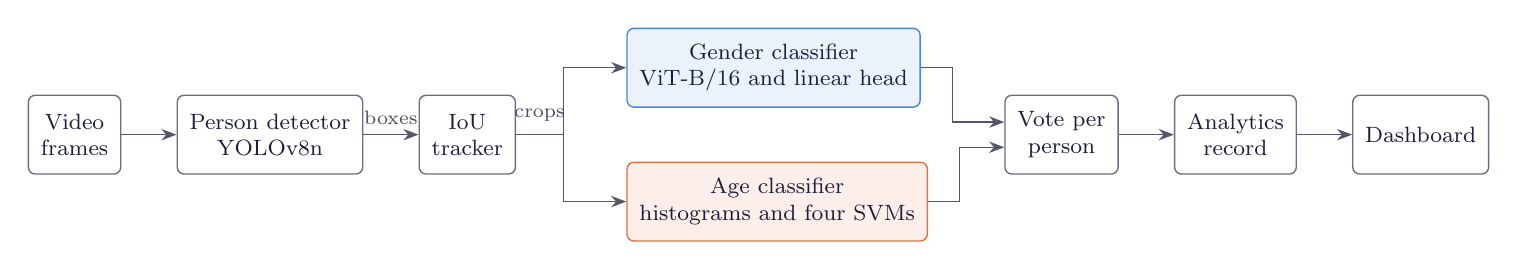
\begin{tikzpicture}[start chain=going right, node distance=7mm]
  \node[box, on chain] (video) {Video\\frames};
  \node[box, on chain] (det) {Person detector\\YOLOv8n};
  \node[box, on chain] (trk) {IoU\\tracker};
  \node[deep, right=14mm of trk, yshift=8.5mm] (gen) {Gender classifier\\ViT-B/16 and linear head};
  \node[classic, right=14mm of trk, yshift=-8.5mm] (age) {Age classifier\\histograms and four SVMs};
  \node[box, right=62mm of trk] (vote) {Vote per\\person};
  \node[box, right=7mm of vote] (rec) {Analytics\\record};
  \node[box, right=7mm of rec] (dash) {Dashboard};

  \draw[flow] (video) -- (det);
  \draw[flow] (det) -- node[note, above] {boxes} (trk);
  \draw[flow] (trk.east) -- ++(6mm,0) |- (gen.west);
  \draw[flow] (trk.east) -- ++(6mm,0) |- (age.west);
  \node[note, above=0.4mm] at ($(trk.east)+(3mm,0)$) {crops};
  \draw[flow] (gen.east) -- ++(4mm,0) |- ($(vote.west)+(0,1.6mm)$);
  \draw[flow] (age.east) -- ++(4mm,0) |- ($(vote.west)+(0,-1.6mm)$);
  \draw[flow] (vote) -- (rec);
  \draw[flow] (rec) -- (dash);
\end{tikzpicture}
\caption{The IFAS pipeline. People are detected and tracked, each tracked person
is classified on several frames by both models, and the pooled labels are written
to one record per video.}
\label{fig:pipeline}
\end{figure*}

\section{System Design}
\label{sec:system}

\subsection{Overview}
Fig.~\ref{fig:pipeline} shows the pipeline and Algorithm~\ref{alg:pipeline} gives
it step by step. A video is read frame by frame. A detector finds people, and a
tracker links the detections that belong to the same person. Crops of each
tracked person go to the gender classifier and the age classifier. Their outputs
are pooled per person. The result is written as one JSON record per video, and
the dashboard reads that file.

\begin{algorithm}[t]
\caption{Processing one video}
\label{alg:pipeline}
\begin{algorithmic}[1]
\Require frames $f_0, f_1, \dots$ at $r$ frames per second; stride $s$; IoU threshold $\tau$; vote gap $g$; vote cap $m$
\Ensure one record per person
\State $A \gets \emptyset$ \Comment{open tracks}
\For{each frame $f_k$ with $k \bmod s = 0$}
  \State $B \gets$ person boxes in $f_k$ with confidence $\geq 0.10$
  \State $P \gets \{(t,b) : t \in A,\ b \in B,\ \mathrm{IoU}(t,b) \geq \tau\}$
  \For{$(t,b) \in P$ in order of falling IoU}
    \If{$t$ and $b$ are both unmatched}
      \State extend $t$ with $b$
    \EndIf
  \EndFor
  \State drop unmatched boxes that lie mostly on a matched person
  \State rejoin an unmatched box to a recently lost track near it
  \State start a track for each remaining box, tentative if below $0.4$
  \State ask the second detector about tentative tracks that persist
  \State close each track unmatched for more than $r$ sampled frames
  \For{each track $t$ matched in $f_k$}
    \If{$t$ is confirmed, has fewer than $m$ votes and its last vote is at least $g$ old}
      \State crop $t$ from $f_k$ and classify gender and age
      \State add both probability vectors to the votes of $t$
    \EndIf
  \EndFor
\EndFor
\State discard unconfirmed tracks and tracks seen in fewer than three frames
\State \Return label, confidence, dwell time and path of each track
\end{algorithmic}
\end{algorithm}

\subsection{Detection and Tracking}
\label{sec:tracking}
We use YOLOv8n restricted to the person class with a confidence threshold of 0.4.
Boxes smaller than $8\times16$ pixels are dropped because they hold too little
detail to classify. Detection runs on every second frame, which halves its cost.

Tracking uses greedy matching on intersection over union (IoU). For two boxes $a$
and $b$,
\begin{equation}
  \mathrm{IoU}(a,b) = \frac{|a \cap b|}{|a \cup b|}.
\end{equation}
Every pair of an open track and a new box with an IoU of at least 0.3 is a
candidate. Candidates are taken in order of falling IoU, and a pair is accepted
if neither side has been matched yet. A track is closed once it has missed as
many sampled frames as the video has frames per second, which is two seconds at
the default stride. Tracks seen in fewer than three frames are treated as
detector noise and discarded.

Two rules keep one person from being counted several times. The first drops a
box when half or more of it lies on a person who is already matched in that
frame, which removes double detections such as a body and its reflection in
glass. The second rejoins lost people. A person cannot vanish in the middle of
the frame, so a track that ends there was lost by the detector. A box with a
confidence of at least 0.25 that appears within one body height of that spot
within 8\,s continues the old track. Near the edges of the frame people do leave
and others arrive, so there a box rejoins a track only if that person was
standing still and the box is in the same place.

The tracker has no appearance model. It is cheap, and Section~\ref{sec:limits}
lists what it cannot do.

\subsection{Weak Detections and the Second Detector}
\label{sec:hunches}
The detector is run with a floor of 0.10, well below the 0.4 needed to start a
track. Boxes in between are used in two ways. A weak box that overlaps a person
already being followed extends that track, since a weak box on a known person is
usually real. A weak box anywhere else opens a tentative track. A tentative
track is followed like any other and counts for nothing.

A tentative track becomes a person in one of two ways. A later box of 0.4 or more
on the same track confirms it. Failing that, once the track has eight
detections a second and larger detector, YOLOv8m, is run on the same frame at
input sizes of 640 and 960 pixels. If it finds a person with a confidence of at
least 0.25 on that spot, the track is confirmed. The question is asked at most
four times per track and at most once a second. A track that is never confirmed
is dropped, and its location is remembered so that the same object is not asked
about again.

A confirmed track keeps its history, so the dwell time of that person starts at
the first weak sighting. If the track began where a known person was lost, the
two are merged.

The reason for this arrangement is cost. Section~\ref{sec:field} shows that the
larger model finds people the small one misses and is six to eleven times
slower. Asking it only about tentative tracks buys most of its benefit for a
small part of its cost.

\subsection{Gender Classifier}
Each crop is resized to $224\times224$ pixels and normalised with the ImageNet
mean and standard deviation. The backbone is ViT-B/16 pretrained on ImageNet-21k,
with 86 million parameters. It splits the crop into 196 patches, adds a class
token and passes the sequence through 12 encoder layers. A pooling layer maps the
class token to a vector of 768 dimensions. One linear layer with 1,538 parameters
maps that vector to two logits, and a softmax turns them into probabilities
(Fig.~\ref{fig:models}a). The loss is cross-entropy.

Training runs in two stages, and each stage has two phases
(Table~\ref{tab:training}). Phase~A is a linear probe. The backbone is frozen and
only the new head is trained, with a learning rate of \sci{-3}. Phase~B unfreezes
the backbone and trains the whole network with a learning rate of \sci{-5}.
Stage~1 runs both phases on PETA. Stage~2 repeats them on labelled crops from the
target store with both learning rates divided by ten, so that the model adapts
without losing what it learned from PETA.

Each phase has its own schedule. The learning rate rises linearly from zero over
the first part of the phase and then falls to zero on a cosine curve
(Fig.~\ref{fig:schedule}). With $T$ steps in the phase and a warmup ratio $w$,
the rate at step $i$ is
\begin{equation}
  \eta_i = \eta_{\max}\cdot
  \begin{cases}
    \dfrac{i}{wT} & i < wT,\\[2.5mm]
    \dfrac{1}{2}\left(1+\cos\dfrac{\pi\,(i-wT)}{T-wT}\right) & i \geq wT.
  \end{cases}
\end{equation}

All runs use AdamW~\cite{loshchilov2019adamw} with a batch size of 64, mixed
precision and gradient clipping at 1.0. Training images are flipped horizontally
with probability 0.5 and receive a small random change in brightness, contrast
and saturation. One tenth of the data is held out for validation with a
stratified split.

\begin{table}[t]
\caption{Training schedule of the gender model}
\label{tab:training}
\centering
\begin{tabular}{@{}llccc@{}}
\toprule
Stage & Phase & Trained & Epochs & Peak rate \\
\midrule
1, PETA  & A, probe     & head          & 4  & \sci{-3} \\
         & B, fine-tune & whole network & 10 & \sci{-5} \\
2, store & A, probe     & head          & 2  & \sci{-4} \\
         & B, fine-tune & whole network & 5  & \sci{-6} \\
\midrule
\multicolumn{5}{@{}l}{AdamW, batch size 64, weight decay 0.3, warmup ratio 0.2,} \\
\multicolumn{5}{@{}l}{gradient clipping at 1.0, mixed precision} \\
\bottomrule
\end{tabular}
\end{table}

\begin{figure}[t]
\centering
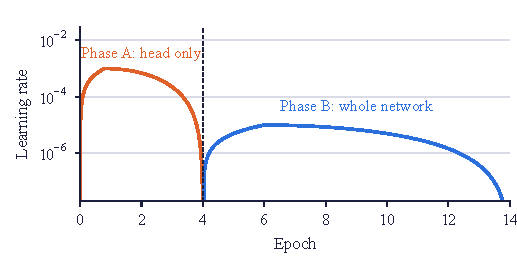
\includegraphics[width=\columnwidth]{lr_schedule.pdf}
\caption{Learning rate over Stage~1 with the selected settings. Each phase warms
up for a fifth of its steps and then decays on a cosine curve. The vertical axis
is logarithmic.}
\label{fig:schedule}
\end{figure}

\begin{figure*}[t]
\centering
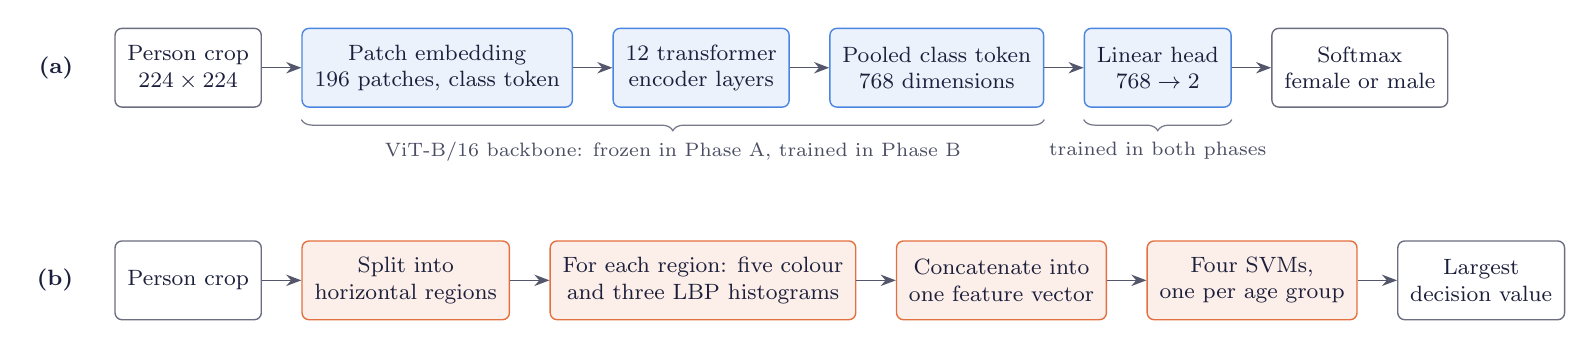
\begin{tikzpicture}[node distance=5mm]
  % (a) gender network
  \begin{scope}[start chain=A going right, every join/.style={flow}]
    \node[box, on chain=A, join] (a1) {Person crop\\$224\times224$};
    \node[deep, on chain=A, join] (a2) {Patch embedding\\196 patches, class token};
    \node[deep, on chain=A, join] (a3) {12 transformer\\encoder layers};
    \node[deep, on chain=A, join] (a4) {Pooled class token\\768 dimensions};
    \node[deep, on chain=A, join] (a5) {Linear head\\$768\rightarrow2$};
    \node[box, on chain=A, join] (a6) {Softmax\\female or male};
  \end{scope}
  \draw[span] ($(a2.south west)+(0,-1.5mm)$) -- ($(a4.south east)+(0,-1.5mm)$)
    node[note, midway, below=4.5pt] {ViT-B/16 backbone: frozen in Phase A, trained in Phase B};
  \draw[span] ($(a5.south west)+(0,-1.5mm)$) -- ($(a5.south east)+(0,-1.5mm)$)
    node[note, midway, below=4.5pt] {trained in both phases};
  \node[font=\footnotesize\bfseries, text=ink, left=4mm of a1] {(a)};

  % (b) age model
  \begin{scope}[start chain=B going right, every join/.style={flow}, yshift=-27mm]
    \node[box, on chain=B, join] (b1) {Person crop};
    \node[classic, on chain=B, join] (b2) {Split into\\horizontal regions};
    \node[classic, on chain=B, join] (b3) {For each region: five colour\\and three LBP histograms};
    \node[classic, on chain=B, join] (b4) {Concatenate into\\one feature vector};
    \node[classic, on chain=B, join] (b5) {Four SVMs,\\one per age group};
    \node[box, on chain=B, join] (b6) {Largest\\decision value};
  \end{scope}
  \node[font=\footnotesize\bfseries, text=ink, left=4mm of b1] {(b)};
\end{tikzpicture}
\caption{The two attribute classifiers. (a) The gender network: a pretrained
ViT-B/16 with a new linear head. (b) The age model: region histograms scored by
one SVM for each age group.}
\label{fig:models}
\end{figure*}

\subsection{Age Classifier}
The age model uses no neural network. Each crop is cut into $R$ horizontal
regions of equal height. With four regions they correspond roughly to the head,
the torso, the upper legs and the lower legs. Two kinds of histogram are computed
for each region. The first is colour: one histogram of $B$ bins for each of the
red, green, blue, hue and saturation channels. The second is texture: one
histogram of uniform LBP codes for each radius in a set $\mathcal{S}$, computed
with $Q$ sampling points and therefore $Q+2$ bins. Every histogram is
L1-normalised. The histograms of all regions are concatenated into one feature
vector (Fig.~\ref{fig:models}b) of length
\begin{equation}
  d = R\,\bigl(5B + |\mathcal{S}|\,(Q+2)\bigr).
  \label{eq:dim}
\end{equation}

One SVM is trained for each of four age groups: 16 to 30, 31 to 45, 46 to 60 and
above 60. Each is a binary classifier that separates its group from the other
three. For every group we search over two kernels. The histogram intersection
kernel is
\begin{equation}
  K(\mathbf{x},\mathbf{y}) = \sum_{i}\min(x_i, y_i),
\end{equation}
and the radial basis function (RBF) kernel is
\begin{equation}
  K(\mathbf{x},\mathbf{y}) = \exp\!\left(-\gamma\,\lVert\mathbf{x}-\mathbf{y}\rVert^{2}\right).
\end{equation}
The search covers $C \in \{0.01, 0.1, 1, 10, 100\}$ for both kernels and
$\gamma \in \{0.001, 0.01, 0.1, 1\}$ for the RBF kernel, 25 settings in all. The
setting with the highest validation mean accuracy is kept for that group. Mean
accuracy for one attribute is
\begin{equation}
  \mA = \frac{1}{2}\left(\frac{\mathit{TP}}{P} + \frac{\mathit{TN}}{N}\right),
  \label{eq:ma}
\end{equation}
where $P$ and $N$ are the numbers of positive and negative examples and
$\mathit{TP}$ and $\mathit{TN}$ are the numbers of each that are classified
correctly. At test time a crop receives the label of the SVM with the largest
decision value.

PETA also labels people under 15. That group has too few examples to train a
stable classifier, and early models underfitted it every time. We left it out.

\subsection{Pooling Predictions per Person}
A single crop can be blurred or partly hidden. A person is visible for many
frames, so IFAS classifies each track several times and combines the answers. A
track is classified at most once every 0.4\,s and at most 12 times in total.
Spacing the samples keeps them from being near copies of one another, and the cap
bounds the cost of a person who stands in view for minutes.

Let $\mathbf{p}_1,\dots,\mathbf{p}_n$ be the probability vectors a model returns
for the $n$ crops of one track. Each crop casts a vote for its most probable
label. The track receives the label $\hat{c}$ with the most votes, and a tie goes
to the label with the higher summed probability. The confidence reported for the
person is the share of the summed probability held by that label,
\begin{equation}
  \mathrm{conf} = \frac{\sum_{j=1}^{n} p_{j,\hat{c}}}{\sum_{j=1}^{n}\sum_{c} p_{j,c}}.
\end{equation}
SVM decision values are passed through a softmax first, so that age confidence is
on the same scale as gender confidence.

\subsection{Analytics and Dashboard}
From each track IFAS takes the time the person was first seen, the time they were
last seen and the dwell time between the two. Dwell time is sorted into the five
tiers of Table~\ref{tab:tiers}. The video is divided into bins of 5\,s. For each
bin the record holds the number of arrivals, the number of exits and the mean and
peak number of people in view. A grid of $16\times9$ cells over the frame
accumulates where people stood, and the frame is split into three vertical zones.

\begin{table}[t]
\caption{Dwell tiers}
\label{tab:tiers}
\centering
\begin{tabular}{@{}lll@{}}
\toprule
Tier & Time in frame & Reading \\
\midrule
Passing  & under 3\,s    & walked through \\
Glancing & 3 to 10\,s    & slowed or looked \\
Browsing & 10 to 30\,s   & stopped \\
Engaged  & 30 to 60\,s   & stayed \\
Dwelling & over 60\,s    & waited or queued \\
\bottomrule
\end{tabular}
\end{table}

Recordings differ in length, so IFAS compares them by rate. Every recording is
split by the clock hours it covers, and each hour $h$ stores the arrivals $a_h$
and the minutes $m_h$ that were watched. The rate for any group $H$ of hours,
such as all Saturdays, is
\begin{equation}
  \rho_H = 60\,\frac{\sum_{h \in H} a_h}{\sum_{h \in H} m_h}
\end{equation}
arrivals per observed hour. A three minute clip then cannot outweigh a three
hour export. A day needs at least five minutes of footage to count, and a trend
is drawn only when three such days exist.

For a coarser summary a recording can also be divided into five equal intervals.
Each interval reports the mean, peak and minimum number of people in view and
the standard deviation of that number. A low standard deviation marks steady
flow and a high one marks a surge. Each interval receives one of six density
labels from Empty to Overcrowded. This labelling is at an earlier stage than the
rest of the system and is not evaluated here.

A dashboard presents the record at two levels of detail. The simple level states
the result in sentences and shows a few headline charts for whoever runs the
store. The detailed level adds filters by gender, age, dwell tier and confidence,
a table of every tracked person and the confidence distributions of both models.

% ---------------------------------------------------------------------------
\section{Experiments}
\label{sec:experiments}

\subsection{Data}
All experiments use PETA~\cite{deng2014peta}. The gender model uses every image
with a gender label, about 19,000 in all, with one tenth held out for validation.

The age model uses the 14,241 images that carry one of the four retained age
labels. Fig.~\ref{fig:agedata} shows how they are spread. The two youngest groups
hold 79\% of the images and the oldest holds 8\%. We split the images into
training, validation and test sets in the proportions of the PETA protocol,
9,500 to 1,900 to 7,600. This gives 7,120 training, 1,424 validation and 5,697
test images. The split is stratified by age group.

\begin{figure}[t]
\centering
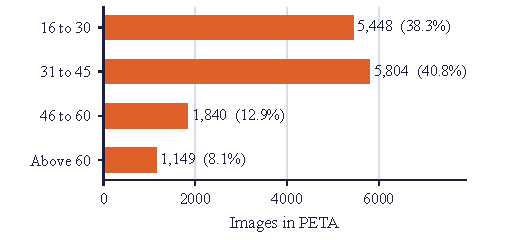
\includegraphics[width=\columnwidth]{age_data.pdf}
\caption{Images per age group among the 14,241 PETA images used for the age
model.}
\label{fig:agedata}
\end{figure}

\subsection{Gender Model}
We varied four settings of Stage~1 one at a time: the backbone learning rate, the
number of linear probe epochs, the weight decay and the warmup ratio.
Table~\ref{tab:gender} lists the values and Fig.~\ref{fig:gender} shows the
results. Schedules were short, between three and seven epochs in total, and each
setting was trained once.

\begin{table}[t]
\caption{Stage 1 settings tested for the gender model}
\label{tab:gender}
\centering
\begin{tabular}{@{}lll@{}}
\toprule
Setting & Values tested & Selected \\
\midrule
Backbone learning rate & \sci{-4}, \sci{-5}, \sci{-7} & \sci{-5} \\
Linear probe epochs & 0, 1, 2, 3, 4 & 4 \\
Weight decay & 0, 0.001, 0.01, 0.05, 0.1, 0.3, 0.5 & 0.3 \\
Warmup ratio & 0, 0.05, 0.1, 0.2, 0.3, 0.4 & 0.2 \\
\bottomrule
\end{tabular}
\end{table}

\begin{figure*}[t]
\centering
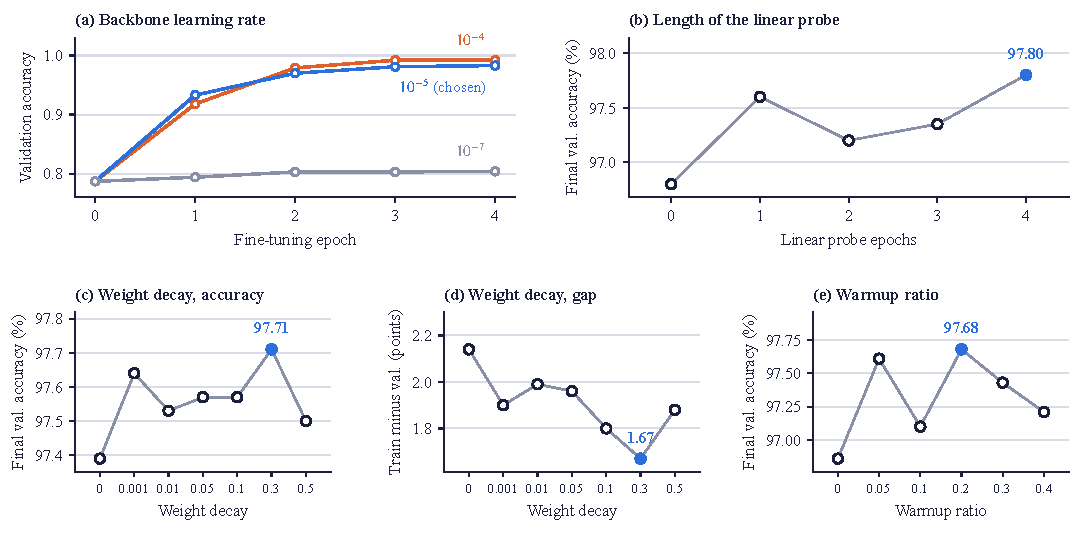
\includegraphics[width=\textwidth]{gender_sensitivity.pdf}
\caption{Sensitivity of the gender model to four training settings on PETA. The
selected value is filled in blue. (a) Validation accuracy during fine-tuning for
three backbone learning rates. Epoch 0 is the end of the linear probe. (b) to (e)
Final validation accuracy, or the gap between training and validation accuracy,
with one setting varied and the rest fixed. Each point is a single run.}
\label{fig:gender}
\end{figure*}

\textit{Learning rate.} With a backbone learning rate of \sci{-7} the model
barely moves. Validation accuracy stays near 0.80, the level the linear probe
reaches alone. Rates of \sci{-4} and \sci{-5} both converge, to 0.992 and 0.983
after four epochs of fine-tuning (Fig.~\ref{fig:gender}a). The higher rate scores
better here, but the run is short. We chose \sci{-5} because a smaller step is
less likely to damage the pretrained features over the longer schedule of the
final model. These runs fine-tuned for one epoch longer than the probing and
weight decay runs, so their accuracy is not comparable with the panels that
follow.

\textit{Linear probe.} Skipping the probe gives the lowest accuracy, 96.8\%. Any
amount of probing helps, and four epochs give the highest accuracy at 97.8\%
(Fig.~\ref{fig:gender}b). The trend is not monotonic, since two epochs score
below one. With one run per setting we read that dip as noise. The training loss
points the other way. Without a probe the loss over the first 200 steps of
fine-tuning falls lower than with one. Lower training loss with lower validation
accuracy is what we would expect if the network fits the training set at the
expense of its pretrained features~\cite{kumar2022finetuning}.

\textit{Weight decay.} Accuracy is lowest without weight decay at 97.39\% and
highest at a decay of 0.3 with 97.71\%. The gap between training and validation
accuracy is also smallest at 0.3: 1.67 points against 2.14 points without decay
(Fig.~\ref{fig:gender}c and~d). The whole range spans a third of a point. The
effect is small, but both measures point the same way.

\textit{Warmup.} Training without warmup gives the lowest accuracy, 96.86\%. A
ratio of 0.2 gives the highest at 97.68\%, with 0.05 close behind at 97.61\%
(Fig.~\ref{fig:gender}e). The values in between follow no clear order.

Taken together, the probe moves accuracy by 1.0 point across its range, warmup
by 0.8 and weight decay by 0.3.

\subsection{Age Model: Feature Settings}
Feature settings were screened on a 30\% subsample of the training and validation
data to keep the search fast. The settings were tuned in the order listed in
Table~\ref{tab:age-config}, and each choice was fixed before the next was tuned.
Fig.~\ref{fig:age} shows the average $\mA$ over the four age groups.

\begin{table}[t]
\caption{Feature settings tested for the age model}
\label{tab:age-config}
\centering
\begin{tabular}{@{}lll@{}}
\toprule
Setting & Values tested & Selected \\
\midrule
Body regions $R$ & 2, 3, 4, 5, 6, 7 & 4 \\
Colour bins $B$ & 8, 16, 24, 32 & 16 \\
LBP points $Q$ & 8, 16, 24 & 16 \\
LBP radii $\mathcal{S}$ & \{1\}, \{1,2\}, \{1,2,3\}, \{1,2,3,4\}, \{2,3\} & \{1,2,3\} \\
Class weight & none, balanced & balanced \\
\bottomrule
\end{tabular}
\end{table}

\begin{figure*}[t]
\centering
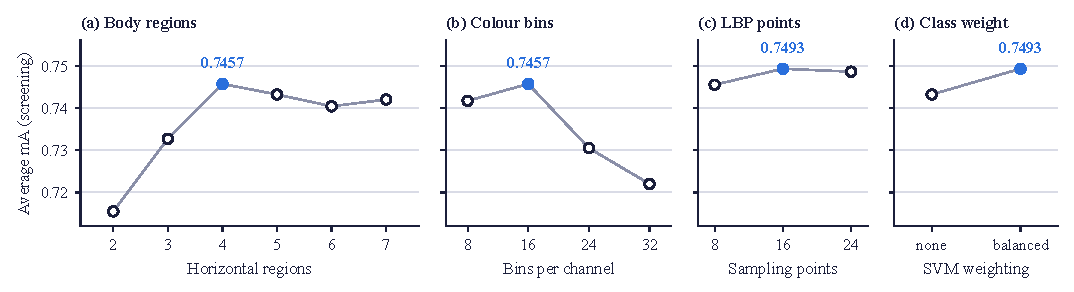
\includegraphics[width=\textwidth]{age_sensitivity.pdf}
\caption{Sensitivity of the age model to its feature settings, measured as
average mA on a 30\% subsample of PETA. All four panels share one vertical scale.
The selected value is filled in blue.}
\label{fig:age}
\end{figure*}

The number of body regions matters most. Average $\mA$ rises from 0.7155 with two
regions to 0.7457 with four and then falls slightly (Fig.~\ref{fig:age}a).
Regions thinner than a quarter of the body hold too few pixels for a stable
histogram. Colour bins behave the same way. Sixteen bins score 0.7457, and 32
bins drop to 0.7220 as the histograms become sparse (Fig.~\ref{fig:age}b). The
number of LBP sampling points has a smaller effect, with 16 points best at 0.7493
(Fig.~\ref{fig:age}c). The five combinations of LBP radii we tried scored within
a narrow band, and radii of 1, 2 and 3 were marginally best. Balanced class
weights raise average $\mA$ from 0.7432 to 0.7493 (Fig.~\ref{fig:age}d), as
expected given the imbalance in Fig.~\ref{fig:agedata}.

\subsection{Age Model: Final Classifiers}
We trained the final SVMs on the full training set in two configurations
(Table~\ref{tab:age-results}). The first is the one released with the pipeline.
It uses five regions and eight LBP points, which by~\eqref{eq:dim} gives 550
features per crop. The second uses the settings selected above, four regions and
16 points, for 536 features. The grid search chose the RBF kernel for every group
in both. The two configurations are close on the validation split, with a mean
$\mA$ of 0.821 and 0.823. The selected one is better for the oldest group, 0.920
against 0.911.

\begin{table}[t]
\caption{Final age classifiers: kernel settings and validation mA}
\label{tab:age-results}
\centering
\begin{tabular}{@{}lcccccc@{}}
\toprule
 & \multicolumn{3}{c}{Released, $d=550$} & \multicolumn{3}{c}{Selected, $d=536$} \\
\cmidrule(lr){2-4}\cmidrule(l){5-7}
Age group & $C$ & $\gamma$ & $\mA$ & $C$ & $\gamma$ & $\mA$ \\
\midrule
16 to 30 & 1  & 1   & 0.7996 & 1  & 1   & 0.8005 \\
31 to 45 & 10 & 1   & 0.7823 & 1  & 1   & 0.7829 \\
46 to 60 & 10 & 0.1 & 0.7897 & 10 & 0.1 & 0.7866 \\
Above 60 & 10 & 0.1 & 0.9108 & 10 & 0.1 & 0.9204 \\
\midrule
Mean     &    &     & 0.8206 &    &     & 0.8226 \\
\bottomrule
\end{tabular}
\end{table}

\subsection{Age Model: Test Results}
The released classifiers were evaluated once on the 5,697 held-out test images.
Table~\ref{tab:age-test} and Fig.~\ref{fig:agetest} give the results. Mean
accuracy is 0.8352 averaged over the four groups, slightly above the validation
figure of 0.8206. The largest change is for the 46 to 60 group, which rises from
0.790 to 0.831.

Read as a single four-way classifier, the model labels 76.7\% of test images
correctly, with a macro-averaged F1 of 0.78. The oldest group is the easiest,
with a precision of 0.90 and a recall of 0.85. The 46 to 60 group is the hardest,
with an F1 of 0.73.

The confusion matrix in Fig.~\ref{fig:agetest}a shows where the errors go. Of the
1,330 misclassified images, 1,057 are placed in a group next to the true one.
That is 79.5\% of all errors. Counting those as near misses, 95.2\% of test
images land in the true group or a neighbouring one. The single largest
confusion is between the two youngest groups: 23\% of people aged 31 to 45 are
labelled 16 to 30, and 14\% the other way.

\begin{table}[t]
\caption{Released age model on the PETA test split}
\label{tab:age-test}
\centering
\begin{tabular}{@{}lccccc@{}}
\toprule
Age group & Images & Precision & Recall & F1 & $\mA$ \\
\midrule
16 to 30 & 2,179 & 0.730 & 0.812 & 0.769 & 0.8107 \\
31 to 45 & 2,322 & 0.794 & 0.720 & 0.755 & 0.7888 \\
46 to 60 & 736   & 0.730 & 0.728 & 0.729 & 0.8312 \\
Above 60 & 460   & 0.897 & 0.848 & 0.872 & 0.9102 \\
\midrule
All      & 5,697 & \multicolumn{3}{c}{accuracy 0.767, macro F1 0.781} & 0.8352 \\
\bottomrule
\end{tabular}
\end{table}

\begin{figure*}[t]
\centering
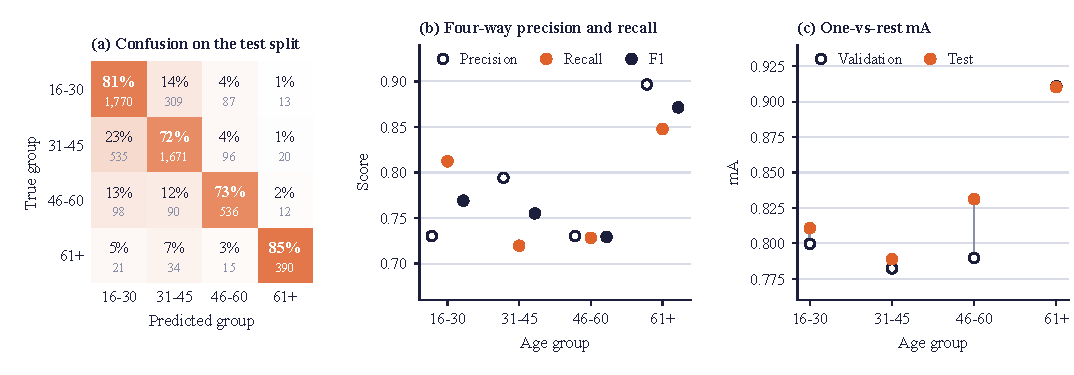
\includegraphics[width=\textwidth]{age_test.pdf}
\caption{The released age model on the PETA test split. (a) Confusion matrix.
Each row sums to 100\%, and the small figure is the number of images. (b)
Precision, recall and F1 when the four SVMs act as one four-way classifier. (c)
One-vs-rest mean accuracy on the validation and test splits.}
\label{fig:agetest}
\end{figure*}

\subsection{Runtime}
\label{sec:runtime}
We timed each stage on a laptop with an AMD Ryzen~3 3250U processor, two cores
and no graphics card. The input was a recording of $848\times478$ pixels, and the
classifiers were timed on the person crops the detector found in it.
Fig.~\ref{fig:runtime} shows the median times.
Detection takes \tDetect\,ms per frame. The age model takes \tAge\,ms per crop,
of which \tAgeFeat\,ms is spent computing histograms. The gender network takes
\tGender\,ms per crop in a batch of 16 and \tGenderOne\,ms for a single crop, and
it dominates the cost. This is why votes are capped. With 12 votes the two
classifiers cost under \tPerson\,s per person on this machine, no matter how long
the person stays in view. Without the cap the cost would grow with dwell time, since
at the default stride a person is detected about a dozen times a second. On a
processor of this class IFAS is a tool for recorded footage. A live feed would
need faster hardware.

\begin{figure}[t]
\centering
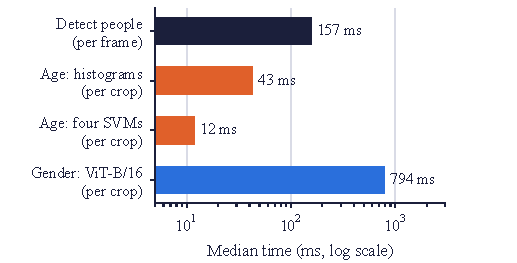
\includegraphics[width=\columnwidth]{runtime.pdf}
\caption{Median time per stage on a two-core laptop processor. The horizontal
axis is logarithmic. Detection is per frame and the classifiers are per person
crop.}
\label{fig:runtime}
\end{figure}

\subsection{Field Check on Shop Footage}
\label{sec:field}
PETA measures the classifiers. It says nothing about detection or tracking, so we
ran the whole pipeline on a recording from outside the dataset: 15\,s of a shop
interior at $1280\times720$ pixels, with glass partitions and stacked boxes. We
labelled it by eye. Five people are in view for the whole clip. A man sits in
the open. A second man walks across the room and works behind a glass partition.
A third person sits at a desk at the left edge of the frame. A fourth sits behind
glass at the back. A fifth stands almost fully hidden behind the third.

\textit{Detection.} Table~\ref{tab:detectors} shows how often four of these
people are detected in 32 evenly spaced frames. The fifth is never detected as a
separate person by any setting. No setting finds everyone. The small model at
its normal threshold never finds the person behind glass. The medium model at
960 pixels finds that person in 44\% of frames and loses the person at the left
desk. At a threshold of 0.05 the small model fires on all four people, but it
also fires on a display stand, and with a higher confidence than on the person
behind glass. A lower threshold alone cannot tell the two apart.

\begin{table}[t]
\caption{Share of 32 frames in which each person is detected at a confidence
of 0.25 or more}
\label{tab:detectors}
\centering
\setlength{\tabcolsep}{3.5pt}
\begin{tabular}{@{}lrcccc@{}}
\toprule
Detector, input size & ms & Seated & Walking & Left desk & Behind glass \\
\midrule
YOLOv8n, 640 & 183   & 100\% & 50\% & 38\% & 0\% \\
YOLOv8s, 640 & 433   & 100\% & 62\% & 6\%  & 0\% \\
YOLOv8s, 960 & 890   & 100\% & 53\% & 3\%  & 12\% \\
YOLOv8m, 640 & 1,057 & 100\% & 72\% & 66\% & 0\% \\
YOLOv8m, 960 & 2,084 & 100\% & 75\% & 25\% & 44\% \\
\midrule
YOLOv8n, 640, at 0.05 & 183 & 100\% & 81\% & 100\% & 100\% \\
\bottomrule
\multicolumn{6}{@{}l}{\footnotesize ms is the time per frame on the laptop of Section~\ref{sec:runtime}. The last row}\\
\multicolumn{6}{@{}l}{\footnotesize also produced 50 boxes that lie on no person.}
\end{tabular}
\end{table}

\textit{Tracking.} Table~\ref{tab:field} compares two versions of the pipeline on
this clip. The first uses IoU matching alone with a single threshold of 0.4. The
second adds the rules of Sections~\ref{sec:tracking} and~\ref{sec:hunches}. The
first version reports five visitors, which happens to equal the true number and
is wrong in every detail. The walking man is counted three times, because the
detector loses him behind the glass. Two people are missed. The mean dwell time
is 4.3\,s for people who were present for 15\,s, and three of five tracks are
labelled as passing through.

The second version reports four visitors, and each is a different real person.
The walking man is one track. The person at the left desk is followed for the
whole clip, and the person behind glass is confirmed by the second detector. The
display stand is opened as a tentative track twice and rejected both times. The
second detector was consulted on 11 of the 188 sampled frames. Processing time
on the laptop rose from 77\,s to 205\,s.

\begin{table}[t]
\caption{The pipeline on the shop clip, before and after the tracking rules.
Each cell is the dwell time reported for that person.}
\label{tab:field}
\centering
\begin{tabular}{@{}lll@{}}
\toprule
Person (present for 15\,s) & IoU matching only & With all rules \\
\midrule
Seated in the open  & 15.0\,s & 15.0\,s \\
Walking, then behind glass & 3.4, 1.5 and 1.0\,s & 14.7\,s \\
At the left desk    & 0.6\,s & 15.0\,s \\
Behind glass at the back & missed & 11.6\,s \\
Hidden behind another & missed & missed \\
\midrule
Tracks reported     & 5 & 4 \\
Distinct people found & 3 of 5 & 4 of 5 \\
Mean dwell time     & 4.3\,s & 14.1\,s \\
\bottomrule
\end{tabular}
\end{table}

This is one clip, chosen because it is hard, and the rules were tuned on it. It
shows what kind of error the first version made and what kind of rule removes
it. It is not a measurement of accuracy. The classifiers also did less well here
than on PETA. Gender was stable for the three people who are clearly visible and
close to a coin toss for the person at the left desk, with a confidence of 0.56.
Age confidence stayed below 0.45 for everyone.

% ---------------------------------------------------------------------------
\section{Discussion}
\label{sec:discussion}

\subsection{Staged Transfer Learning}
The probing result agrees with Kumar et al.~\cite{kumar2022finetuning}. A new head
starts with random weights, and its first gradients are large and carry little
information. If the backbone is trainable at that point those gradients flow into
it. Training the head alone first removes the problem at the cost of a few short
epochs.

The preferred weight decay of 0.3 is higher than the range of 0.01 to 0.1 often
used with AdamW. PETA has 19,000 images and ViT-B/16 has 86 million parameters,
so a need for stronger regularisation is plausible. The measured differences are
small, and each rests on one run. Repeating the study with several random seeds
is the first thing we would do with more compute.

\subsection{Reading the Age Results}
The oldest group is the easiest on every measure. Grey or white hair changes the
colour histogram of the top region, and posture and clothing may add to the
signal. This is our reading of the result. We did not test which features carry
it.

The two youngest groups are confused with each other more than any other pair. A
person of 29 and a person of 32 fall on opposite sides of a boundary and look
alike at surveillance resolution. The confusion matrix supports this view of the
errors as boundary effects. Four errors in five are off by one group, and errors
of two or three groups make up 4.8\% of the test set. For a store that wants a
rough age profile of its visitors, an error of one group matters far less than
an error of three. A measure that respects the order of the groups would credit
the model for this, and mean accuracy does not.

The oldest group has only 8\% of the data and still reaches a recall of 0.85.
Balanced class weights push each SVM to find its positives, and this result
suggests they are doing that job.

Leaving out the under 15 group reflects a wider problem. Surveillance datasets
hold few children, both because few appear in the footage and because privacy
rules limit how such data is collected. A store that needs to know how many
children visit should not rely on IFAS for that.

\subsection{Feature Settings and the Released Model}
The released model and the selected settings differ in two ways, the number of
regions and the number of LBP points. On validation data the difference in mean
$\mA$ is 0.002, which is too small to separate the two on a single split. The
screening study still earns its place. It shows that the model is not fragile.
Across every setting we tried, average $\mA$ stays between 0.7155 and 0.7493, a
spread of 3.4 points, and the two settings that cost most are too few body
regions and too many colour bins.

\subsection{Why Two Kinds of Model}
One network that predicts gender and age together would be simpler to deploy. We
kept the two apart for two reasons. The age model reproduces a published
baseline, so its numbers can be set directly against those of Deng et
al.~\cite{deng2014peta}. Its features can also be inspected, since a histogram bin
is a colour range in a named part of the body. The gender task has enough data to
train a large network, and the accuracy of the transformer there is hard to match
with hand-built features.

The runtime figures add a third argument. The age model costs less than a
tenth of the gender network per crop on a processor. A store with no graphics
card can run age on every crop and spend its budget on gender.

\subsection{Limitations}
\label{sec:limits}
Apart from the field check, the numbers in this paper come from PETA. The field
check is one clip of 15\,s labelled by eye, so accuracy in a real store is still
unmeasured. Several other limits follow from the design.
\begin{itemize}
  \item The tracker does not re-identify people by appearance. A person who
        leaves the frame and returns is counted twice, and two people who cross
        can swap tracks. The rule that rejoins lost tracks is a heuristic and
        can merge two people who stand in the same spot a few seconds apart.
  \item A person no detector finds is never counted. In the field check one
        person of five, hidden behind another, was missed for the whole clip.
  \item The tracking rules were tuned on a single recording. They need to be
        checked on labelled footage from other stores.
  \item Occupancy is the number of people in view, not the number in the store.
  \item Dwell time measures presence in the frame. It stands in for interest and
        does not measure it.
  \item The age SVMs were trained at the resolution of PETA images. Small or
        blurred crops receive labels with low confidence.
  \item Accuracy per track has not been measured. Pooling helps only when the
        errors on different frames are independent.
  \item The gender results are validation accuracy from short single runs. The
        gender model has no held-out test result yet.
  \item The runtime figures come from one processor and one recording.
\end{itemize}

% ---------------------------------------------------------------------------
\section{Conclusion}
\label{sec:conclusion}

IFAS turns store footage into a record of who came in, when they came and how
long they stayed. It does so with a mix of models chosen task by task: a small
detector for speed, a fine-tuned transformer for gender and an SVM baseline for
age. On PETA the gender model reaches 97.8\% validation accuracy. The age model
reaches a mean $\mA$ of 0.835 on the test split, and 95\% of its predictions are
within one age group of the truth. The sensitivity study shows that linear
probing before fine-tuning has the largest effect on the gender model and that
the number of body regions has the largest effect on the age model. The timings
show that the gender network accounts for most of the cost and that capping the
votes per person keeps that cost bounded. On a hard clip from outside PETA,
rejoining lost tracks and checking weak detections with a second detector
raised the number of people found from three of five to four of five and
brought the reported dwell times in line with the footage.

Three pieces of work come next. The first is to label store footage and measure
accuracy per track on it. The second is to add re-identification so that
returning visitors are counted once. The third is to run the pipeline on a live
camera feed, which we have not yet tested.

\section*{Acknowledgment}
The authors thank Prof. Neha Katre for guidance throughout this project.

\bibliographystyle{IEEEtran}
\bibliography{refs}

\end{document}
